\documentclass[12pt]{article}
\usepackage[english]{babel}
\usepackage[utf8]{inputenc}
\usepackage{amsmath, amssymb,amsthm}
\usepackage{graphicx}
\usepackage{hyperref}
\usepackage{geometry}
\usepackage{xcolor}

\graphicspath{{./images/}}
\setlength{\topmargin}{0pt}
\setlength{\headsep}{0pt}
\textheight = 600pt

\title{Probability Theory \\ Daily Task}
\author{Ben Kallus}
\date{October 26, 2020}

\begin{document}
\color{white}
\pagecolor{black}
\maketitle

\begin{align*}
    f_{X,Y}(x,y) &= \begin{cases} 6 & x^2 \leq y \leq x, \\ 0 & \text{else.} \end{cases}
\end{align*}

\noindent{\bf 1.}
\begin{center}
    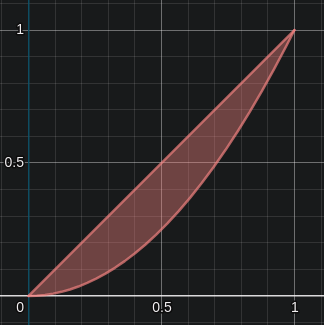
\includegraphics{capture0.png}
\end{center}

\medskip
\noindent{\bf 2.}
\begin{align*}
    f_X(x) &= \begin{cases} 6(\sqrt x - x) & 0 \leq x \leq 1, \\ 0 & \text{else.} \end{cases} \\
    f_Y(y) &= \begin{cases} 6(y - y^2) & 0 \leq y \leq 1, \\ 0 & \text{else.} \end{cases}
\end{align*}

$X$ and $Y$ are not independent, since $f_X(\frac12)f_Y(\frac12) \approx 1.864$ and $f_{X,Y}(\frac12, \frac12) = 6$.

\medskip
\noindent{\bf 3.}
\begin{align*}
    \mathbb E[XY] &= \int\limits_{0}^1 \int\limits_{x^2}^x 6xy \,dy \,dx \\
                  &= \frac14.
\end{align*}

\medskip
\noindent{\bf 4.}
\begin{align*}
    f_{X|Y}(x|5) &= \frac{f_{X,Y}(x,0.5)}{f_Y(0.5)} \\
                 &= \frac{2f_{X,Y}(x,0.5)}{3}
\end{align*}

\end{document}